% Options for packages loaded elsewhere
\PassOptionsToPackage{unicode}{hyperref}
\PassOptionsToPackage{hyphens}{url}
%
\documentclass[
  10pt,
  ignorenonframetext,
]{beamer}
\usepackage{pgfpages}
\setbeamertemplate{caption}[numbered]
\setbeamertemplate{caption label separator}{: }
\setbeamercolor{caption name}{fg=normal text.fg}
\beamertemplatenavigationsymbolsempty
% Prevent slide breaks in the middle of a paragraph
\widowpenalties 1 10000
\raggedbottom
\setbeamertemplate{part page}{
  \centering
  \begin{beamercolorbox}[sep=16pt,center]{part title}
    \usebeamerfont{part title}\insertpart\par
  \end{beamercolorbox}
}
\setbeamertemplate{section page}{
  \centering
  \begin{beamercolorbox}[sep=12pt,center]{part title}
    \usebeamerfont{section title}\insertsection\par
  \end{beamercolorbox}
}
\setbeamertemplate{subsection page}{
  \centering
  \begin{beamercolorbox}[sep=8pt,center]{part title}
    \usebeamerfont{subsection title}\insertsubsection\par
  \end{beamercolorbox}
}
\AtBeginPart{
  \frame{\partpage}
}
\AtBeginSection{
  \ifbibliography
  \else
    \frame{\sectionpage}
  \fi
}
\AtBeginSubsection{
  \frame{\subsectionpage}
}
\usepackage{lmodern}
\usepackage{amssymb,amsmath}
\usepackage{ifxetex,ifluatex}
\ifnum 0\ifxetex 1\fi\ifluatex 1\fi=0 % if pdftex
  \usepackage[T1]{fontenc}
  \usepackage[utf8]{inputenc}
  \usepackage{textcomp} % provide euro and other symbols
\else % if luatex or xetex
  \usepackage{unicode-math}
  \defaultfontfeatures{Scale=MatchLowercase}
  \defaultfontfeatures[\rmfamily]{Ligatures=TeX,Scale=1}
\fi
% Use upquote if available, for straight quotes in verbatim environments
\IfFileExists{upquote.sty}{\usepackage{upquote}}{}
\IfFileExists{microtype.sty}{% use microtype if available
  \usepackage[]{microtype}
  \UseMicrotypeSet[protrusion]{basicmath} % disable protrusion for tt fonts
}{}
\makeatletter
\@ifundefined{KOMAClassName}{% if non-KOMA class
  \IfFileExists{parskip.sty}{%
    \usepackage{parskip}
  }{% else
    \setlength{\parindent}{0pt}
    \setlength{\parskip}{6pt plus 2pt minus 1pt}}
}{% if KOMA class
  \KOMAoptions{parskip=half}}
\makeatother
\usepackage{xcolor}
\IfFileExists{xurl.sty}{\usepackage{xurl}}{} % add URL line breaks if available
\IfFileExists{bookmark.sty}{\usepackage{bookmark}}{\usepackage{hyperref}}
\hypersetup{
  pdftitle={HWSE path analysis},
  hidelinks,
  pdfcreator={LaTeX via pandoc}}
\urlstyle{same} % disable monospaced font for URLs
\newif\ifbibliography
\setlength{\emergencystretch}{3em} % prevent overfull lines
\providecommand{\tightlist}{%
  \setlength{\itemsep}{0pt}\setlength{\parskip}{0pt}}
\setcounter{secnumdepth}{-\maxdimen} % remove section numbering
%---------------------------------------------------------------------------
% BeamerHead.sty
%---------------------------------------------------------------------------
\usepackage{ifxetex,ifluatex}

%---------------------------------------------------------------------------
% General
%---------------------------------------------------------------------------
\usepackage{setspace}
\setstretch{1.25}

%\usepackage[T1]{fontenc} % Use 8-bit encoding that has 256 glyphs
% \usepackage[utf8]{inputenc}
% \usepackage{lmodern}

%\usepackage{fourier} % Use the Adobe Utopia font for the document - comment this line to return to the LaTeX default

% \setbeamerfont{item}{size*={7.5}{8}}
% \setbeamerfont{item projected}{size*={7.5}{8}}
% \setbeamerfont{itemize item}{size*={7.5}{8}}
% \setbeamerfont{itemize subitem}{size*={7.5}{8}}
% \setbeamerfont{itemize subsubitem}{size*={7.5}{8}}
% \setbeamerfont{itemize/enumerate body}{size*={7.5}{8}}
% \setbeamerfont{itemize/enumerate subbody}{size*={7.5}{8}}
% \setbeamerfont{itemize/enumerate subsubbody}{size*={7.5}{8}}
% \setbeamerfont{caption}{size*={7.5}{8}}
% \setbeamerfont{caption name}{size*={7.5}{8}}
% \setbeamerfont{frametitle}{size*={9}{9.5}}
% \setbeamerfont{normal text}{size*={7.5}{8}}
% Smaller itemize bullets
\setbeamertemplate{itemize items}{
	\raisebox{0.15\height}{$\vcenter{\hbox{\scalebox{0.5}{
	\usebeamercolor[fg]{structure} $\blacktriangleright$}}}$}}

%\usepackage{sectsty} % Allows customizing section commands
%\allsectionsfont{\centering \normalfont\scshape} % Make all sections centered, the default font and small caps
%\numberwithin{equation}{section} % Number equations within sections
%\numberwithin{figure}{section} % Number figures within sections
%\numberwithin{table}{section} % Number tables within sections

\usepackage{multicol}
\setlength{\columnsep}{20pt}
\newlength\Colsep

%---------------------------------------------------------------------------
% Header/footer
%---------------------------------------------------------------------------
\setbeamertemplate{navigation symbols}{}
\setbeamertemplate{footline}[page number]

%---------------------------------------------------------------------------
% Citations
%---------------------------------------------------------------------------
% \usepackage[backend=bibtex]{biblatex}

%---------------------------------------------------------------------------
% Tables, figures, images
%---------------------------------------------------------------------------
\usepackage{wrapfig}
\usepackage{longtable}
\setlength{\LTcapwidth}{\textwidth}
\usepackage{xtab, booktabs}
\usepackage{multirow}

\usepackage{tikz}% Probability trees and flow charts and the like
\usetikzlibrary{%
trees,
arrows,
shapes,
%decoration,
automata,
backgrounds,
petri}

% Witin cell wrapping
% https://tex.stackexchange.com/questions/2441/how-to-add-a-forced-line-break-inside-a-table-cell
\usepackage{makecell}
\renewcommand\theadalign{bc}
\renewcommand\theadfont{\bfseries}
\renewcommand\theadgape{\Gape[4pt]}
\renewcommand\cellgape{\Gape[4pt]}
% Usage
% \thead{Two line \\ head}
% \makecell{Some really \\ longer text}

% \usepackage{graphicx,grffile}
% For tables and figures in parts %%%%
\usepackage{caption}
\DeclareCaptionLabelFormat{cont}{#1~#2\alph{ContinuedFloat}}
% \usepackage{subcaption}
% \captionsetup{font=scriptsize,labelfont=scriptsize}
%\graphicspath{ {file.path.here} }

% \usepackage{subfloat}

% Set column widths in tabular environment!
\usepackage{array}
\newcommand{\PreserveBackslash}[1]{\let\temp=\\#1\let\\=\temp}
\newcolumntype{C}[1]{>{\PreserveBackslash\centering}p{#1}}
\newcolumntype{R}[1]{>{\PreserveBackslash\raggedleft}p{#1}}
\newcolumntype{L}[1]{>{\PreserveBackslash\raggedright}p{#1}}

% Fancy fit image command with optional caption
\usepackage{adjustbox} % Shrink stuff
% \usepackage{showframe} % Useful for debugging

%---------------------------------------------------------------------------
% Typographical addendum
%---------------------------------------------------------------------------
\usepackage{bbm} % more BB
\input{\string~/HeadRs/common_supplement.tex}

\title{HWSE path analysis}
\subtitle{Cancer incidence}
\author{}
\date{\vspace{-2.5em}\today}

\begin{document}
\frame{\titlepage}

\begin{frame}{From Erika Garcia's paper\textsuperscript{1}}
\protect\hypertarget{from-erika-garcias-papergarcia_2017}{}

\begin{figure}[H]\begin{center}
\fbox{
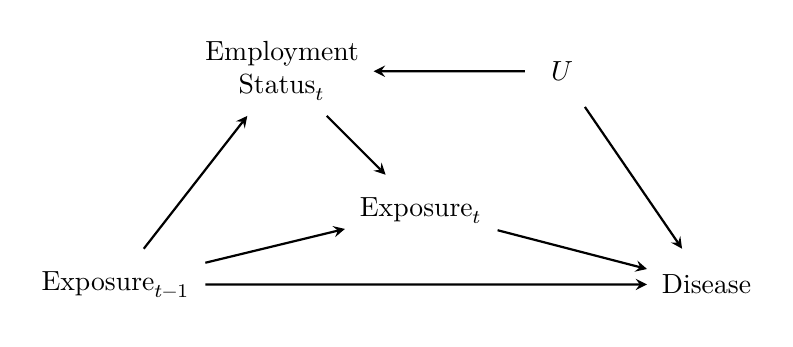
\begin{tikzpicture}[>= stealth, auto,
node distance = 2.5cm, semithick, scale=0.85,
thick, fill=white, inner sep=5pt]
\tikzstyle{every state}=[
shape = rectangle, align = center, draw = none
]
\node[state] (employment) {Employment\\Status$_t$};
\node[state] (E1) [below left of=employment, shift=({250:1cm})] {Exposure$_{t - 1}$};
\node[state] (E) [below right of=employment]{Exposure$_{t}$};
\node[state] (D) [right of=E1, node distance=7.5cm] {Disease};
\node[state] (U) [above right of=E] {$U$};
\path[->] (U) edge (employment);
\path[->] (E1) edge (employment);
\path[->] (U) edge (D);
\path[->] (employment) edge (E);
\path[->] (E1) edge (E);
\path[->] (E) edge (D);
\path[->] (E1) edge (D);
\end{tikzpicture}
}
\end{center}
\end{figure}

The presence of the healthy worker survivor effect (HWSE) implies the
presence of the following three conditions:

\begin{enumerate}
\tightlist
\item
  Leaving work predicts (future) exposure
\item
  Leaving work is associated with the disease
\item
  Prior exposure predicts predicts leaving work
\end{enumerate}

\end{frame}

\begin{frame}{Analytic population}
\protect\hypertarget{analytic-population}{}

\begin{itemize}
\tightlist
\item
  Cancer incidence follow-up

  \begin{itemize}
  \tightlist
  \item
    Starting in 1973 in plants 1 and 2; 1985 in plant 3
  \item
    Ending in 2015
  \end{itemize}
\item
  Employment records in in 1994; individuals still at work in 1995 were
  censored
\end{itemize}

\end{frame}

\begin{frame}{2. Leaving work and cancer incidence}
\protect\hypertarget{leaving-work-and-cancer-incidence}{}

\begin{figure}[H]\begin{center}
\fbox{
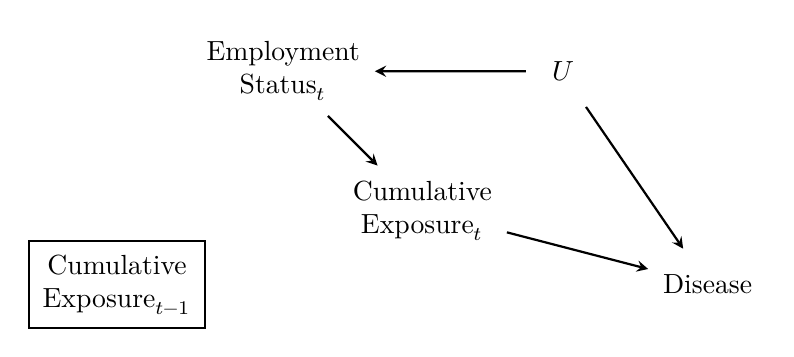
\begin{tikzpicture}[>= stealth, auto,
node distance = 2.5cm, semithick, scale=0.85,
thick, fill=white, inner sep=5pt]
\tikzstyle{every state}=[
shape = rectangle, align = center, draw = none
]
\node[state] (employment) {Employment\\Status$_t$};
\node[state] (E1) [below left of=employment, shift=({250:1cm}),draw=black] {Cumulative\\Exposure$_{t - 1}$};
\node[state] (E) [below right of=employment]{Cumulative\\Exposure$_{t}$};
\node[state] (D) [right of=E1, node distance=7.5cm] {Disease};
\node[state] (U) [above right of=E] {$U$};
\path[->] (U) edge (employment);
%\path[->] (E1) edge (employment);
\path[->] (U) edge (D);
\path[->] (employment) edge (E);
%\path[->] (E1) edge (E);
\path[->] (E) edge (D);
%\path[->] (E1) edge (D);
\end{tikzpicture}
}
\end{center}
\end{figure}

\begin{itemize}
\tightlist
\item
  Exposure: Employment status (binary)
\item
  Conditioning set:
\end{itemize}

\begin{columns}
\begin{column}{0.55\linewidth}
\begin{itemize}\item[]\begin{itemize}
\item Age (index time for Cox model)
\item Cumulative MWF exposure (lagged 1 year)
\item Year of hire
\end{itemize}\end{itemize}
\end{column}
\begin{column}{0.45\linewidth}
\begin{itemize}\item[]\begin{itemize}
\item Race (MI)
\item Plant
\item Sex
\end{itemize}\end{itemize}
\end{column}
\end{columns}

\end{frame}

\begin{frame}{2. Leaving work at age 60 and cancer incidence}
\protect\hypertarget{leaving-work-at-age-60-and-cancer-incidence}{}

\[\begin{aligned}
\log h(t \mid a,\ x)
& = \log h_0 (t) \\ & \hspace{2em}
+ a \cdot \Ind{t < 60} \cdot \beta_1
+ a \cdot \Ind{t \ge 60} \cdot \beta_2 \\ & \hspace{2em}
+ x \begin{pmatrix}\beta_3 & \cdots & \beta_p\end{pmatrix}^\top
\end{aligned}\]

where \(a\) is the indicator of having left work, \(t\) is age, and
\(x\) is a vector of covariates

\begin{itemize}
\tightlist
\item
  Coefficients \(\beta_1\) and \(\beta_2\) may be thought of as
  interaction effects of employment status and age
\end{itemize}

\end{frame}

\begin{frame}{3. Prior exposure and leaving work}
\protect\hypertarget{prior-exposure-and-leaving-work}{}

\begin{figure}[H]\begin{center}
\fbox{
\begin{tikzpicture}[>= stealth, auto,
node distance = 2.5cm, semithick, scale=0.85,
thick, fill=white, inner sep=5pt]
\tikzstyle{every state}=[
shape = rectangle, align = center, draw = none
]
\node[state] (employment) {Employment\\Status$_t$};
\node[state] (E1) [below left of=employment, shift=({250:1cm})] {Exposure$_{t - 1}$};
\node[state] (E) [below right of=employment]{};
\node[state] (D) [right of=E1, node distance=7.5cm] {};
\node[state] (U) [above right of=E] {};
%\path[->] (U) edge (employment);
\path[->] (E1) edge (employment);
%\path[->] (U) edge (D);
%\path[->] (employment) edge (E);
%\path[->] (E1) edge (E);
%\path[->] (E) edge (D);
%\path[->] (E1) edge (D);
\end{tikzpicture}
}
\end{center}
\end{figure}

\begin{itemize}
\tightlist
\item
  Exposure: Cumulative exposure lagged 1 year
\item
  Conditioning set:
\end{itemize}

\begin{columns}
\begin{column}{0.55\linewidth}
\begin{itemize}\item[]\begin{itemize}
\item Age (index time for Cox model)
\item Year of hire
\item Race (MI)
\end{itemize}\end{itemize}
\end{column}
\begin{column}{0.45\linewidth}
\begin{itemize}\item[]\begin{itemize}
\item Plant
\item Sex
\end{itemize}\end{itemize}
\end{column}
\end{columns}

\end{frame}

\begin{frame}{Citations}
\protect\hypertarget{citations}{}

\hypertarget{refs}{}
\leavevmode\hypertarget{ref-Garcia_2017}{}%
1. Garcia E, Picciotto S, Costello S, Bradshaw PT, Eisen EA. Assessment
of the healthy worker survivor effect in cancer studies of the united
autoworkers-general motors cohort. \emph{Occupational and environmental
medicine}. 2017;74(4):294-300.

\end{frame}

\end{document}
